\chapter{Gestion des Utilisateurs et des Comptes bancaires (Administrateur)}

\section{Gestion des utilisateurs}\label{gestion_users}
L'administrateur a accès à la gestion des utilisateurs qui utilisent le Portail Pro.one.be. Il existe trois profils différents: l’administrateur, le gestionnaire des utilisateurs et le gestionnaire des données de l’activité.

\subsection{Les trois types de profils}
Le profil \textbf{administrateur} a accès à toutes les fonctionnalités:
\begin{itemize}
    \item Consulter et modifier toutes les données du pouvoirs organisateur: données des structures d’accueil, données du personnel, données des services autres, données des profils utilisateurs;
    \item Créer, désactiver ou activer, supprimer les profils utilisateurs.
\end{itemize}

Le profil \textbf{gestionnaire des utilisateurs} peut uniquement: créer, désactiver ou activer, supprimer les profils utilisateurs du pouvoir organisateur. Nous lui (ou leur) recommandons de vérifier régulièrement si la liste est à jour, si tous les profils qui doivent être désactivés ou supprimés le sont bien.

Le profil \textbf{gestionnaires des données de l’activité} peut:
\begin{itemize}
    \item Consulter et modifier toutes les données du milieu d’accueil de la petite enfance, du secteur de l’accueil temps libre et du service PSE auxquels l'administrateur lui a donné accès.
    \item Pour le secteur de l’accueil petite enfance, l’accès se donne par milieu d’accueil.
    \item Pour l’accueil temps libre, l’accès se donne par secteur (AES de type 1, AES de type 2, EDD, CDV).
    \item Pour les PSE, l’accès se donne par service.
\end{itemize}

\subsection{Ajouter un nouvel utilisateur}
Pour ajouter un utilisateur, dans le volet de navigation à gauche, développez le volet \ovalbox{Administration}, puis cliquez sur l'entrée \ovalbox{Utilisateurs}. L'écran vous présentera la liste des utilisateurs. 

Pour ajouter un utilisateur, cliquez sur le bouton \ovalbox{Ajouter un utilisateur}.

\vspace{2mm}
\centerline{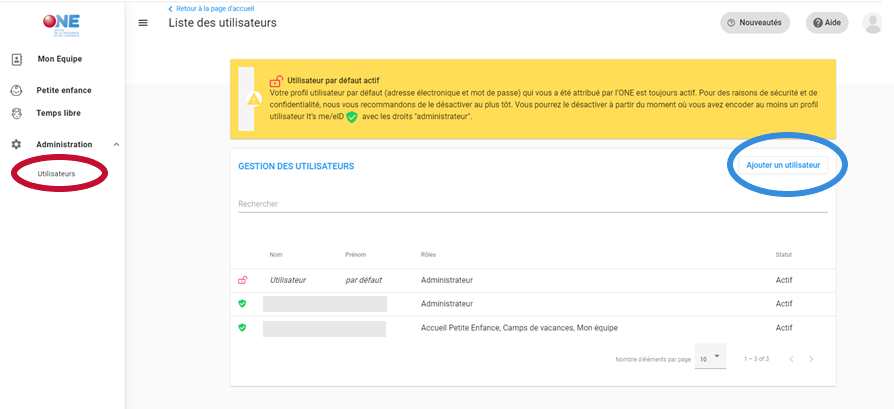
\includegraphics[width=15cm]{Images/intro/gestion_user.png}}

Une petite fenêtre s'ouvre et vous invite à renseigner le nom, prénom et numéro national de la personne. Cliquez ensuite sur \ovalbox{Ajouter l'utilisateur}

\vspace{2mm}
\centerline{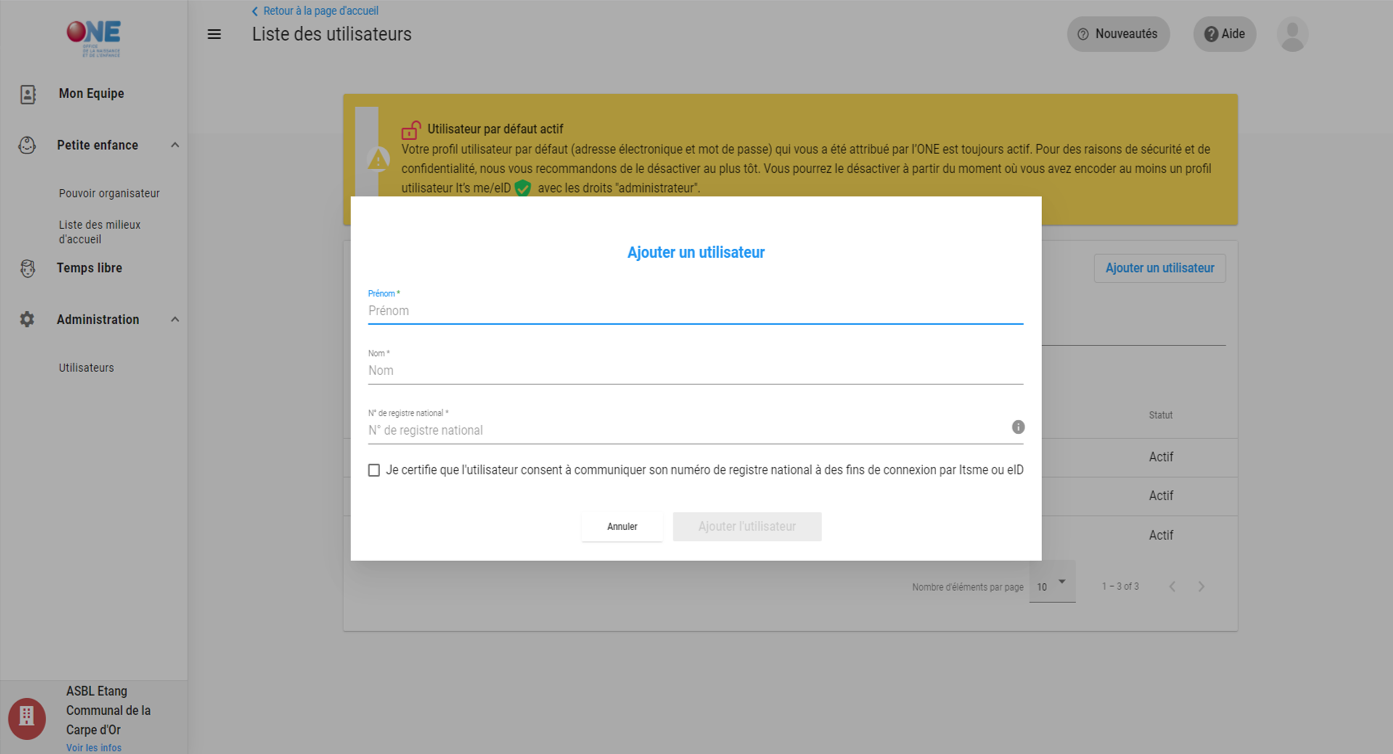
\includegraphics[width=15cm]{Images/intro/ajout_user.png}}
Configurez ensuite les droits de l'utilisateur en cochant les secteurs pour lesquels vous souhaitez accorder un accès. Si vous souhaitez donner les droits d'administrateur, glissez le bouton \textbf{Administrateur}. Cliquez ensuite sur le bouton \ovalbox{Enregistrer} pour sauvegarder vos modifications. 

La "\textbf{Gestion des utilisateurs}" permet d’accorder à cette personne la gestion de droits d'accès (créer, supprimer, désactiver ou activer un profil utilisateur).


\vspace{2mm}
\centerline{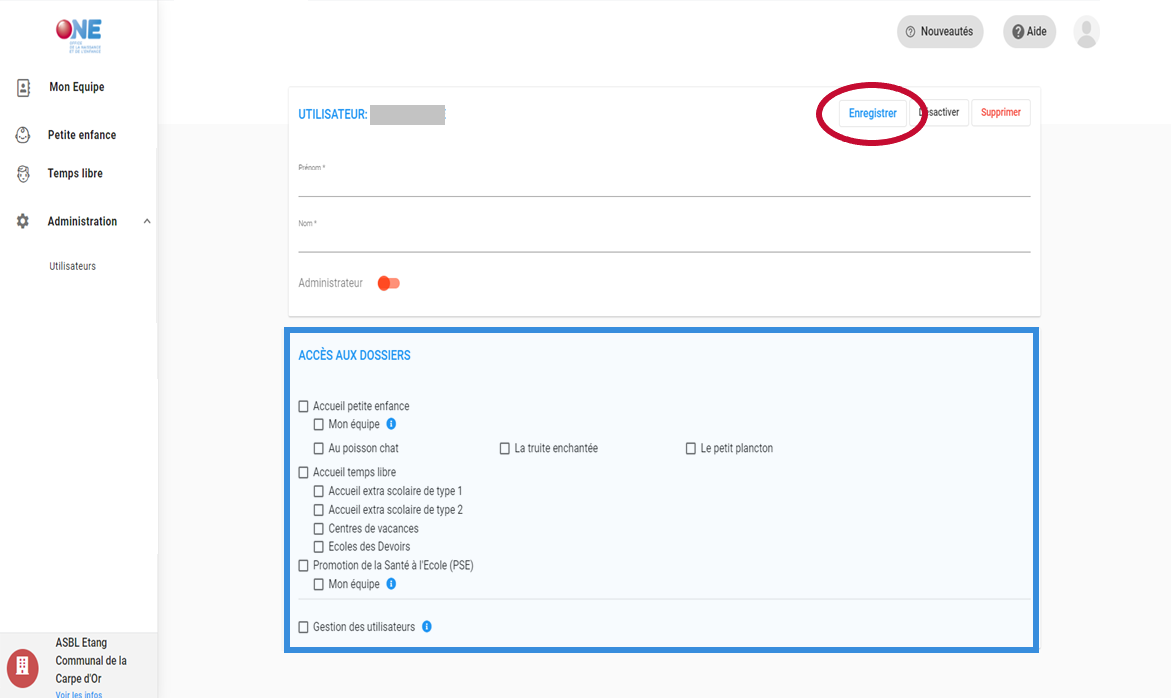
\includegraphics[width=8cm]{Images/intro/config_user.png}\hspace{1cm}  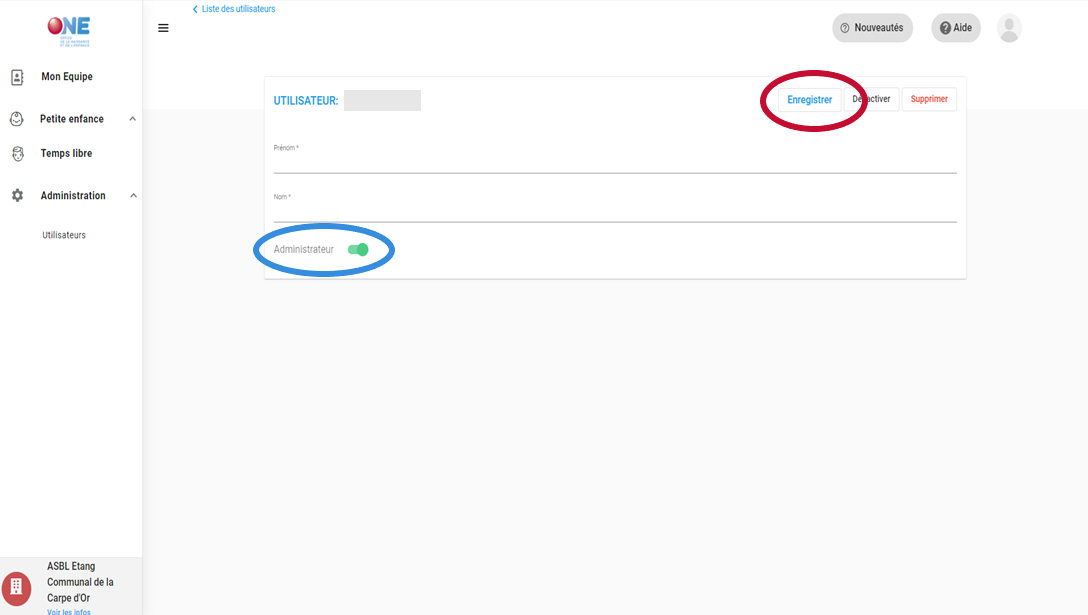
\includegraphics[width=8cm]{Images/intro/config_admin.png}}

\vspace{2mm}

Les utilisateurs qui apparaissent dans la liste pourront se connecter au Portail Pro.one.be via It's me ou eID. Nous vous conseillons de mettre à jour cette liste (ajout ou retrait de droits, suppression ou création d'utilisateur, etc). Configurez ensuite les droits de l'utilisateur en cochant les secteurs pour lesquels vous souhaitez accorder un accès. Les personnes pourront consulter et modifier uniquement les sections pour lesquelles vous avez octroyé les droits d'accès. 

Le bouton \ovalbox{Supprimer} vous permet de supprimer définitivement un profil (par exemple si la personne ne fait plus partie de l'organisation). Cette personne ne pourra plus se connecter à votre portail une fois son profil supprimé.

Le bouton \ovalbox{Désactiver} vous permet de désactiver temporairement le profil d’un personne (par exemple si la personne est en maladie de longue durée). Mais son profil reste dans la liste des profils et vous pourrez le réactiver à tout moment.


\section{Gestion des comptes bancaires}
Pour accéder à la gestion de vos données bancaires, développez le volet \ovalbox{Accueil Temps Libre}, puis cliquez sur l'entrée \ovalbox{Comptes et données}. Vous serez dirigé vers la Signalétique de votre Pouvoir organisateur. Cliquez ensuite sur l'onglet "Comptes bancaires". Vous aurez l'occasion d'ajouter ou de modifier vos numéros de comptes. 

\begin{figure}[!h]
    \centering
    \begin{subfigure}[t]{0.48\textwidth}
         \centering
         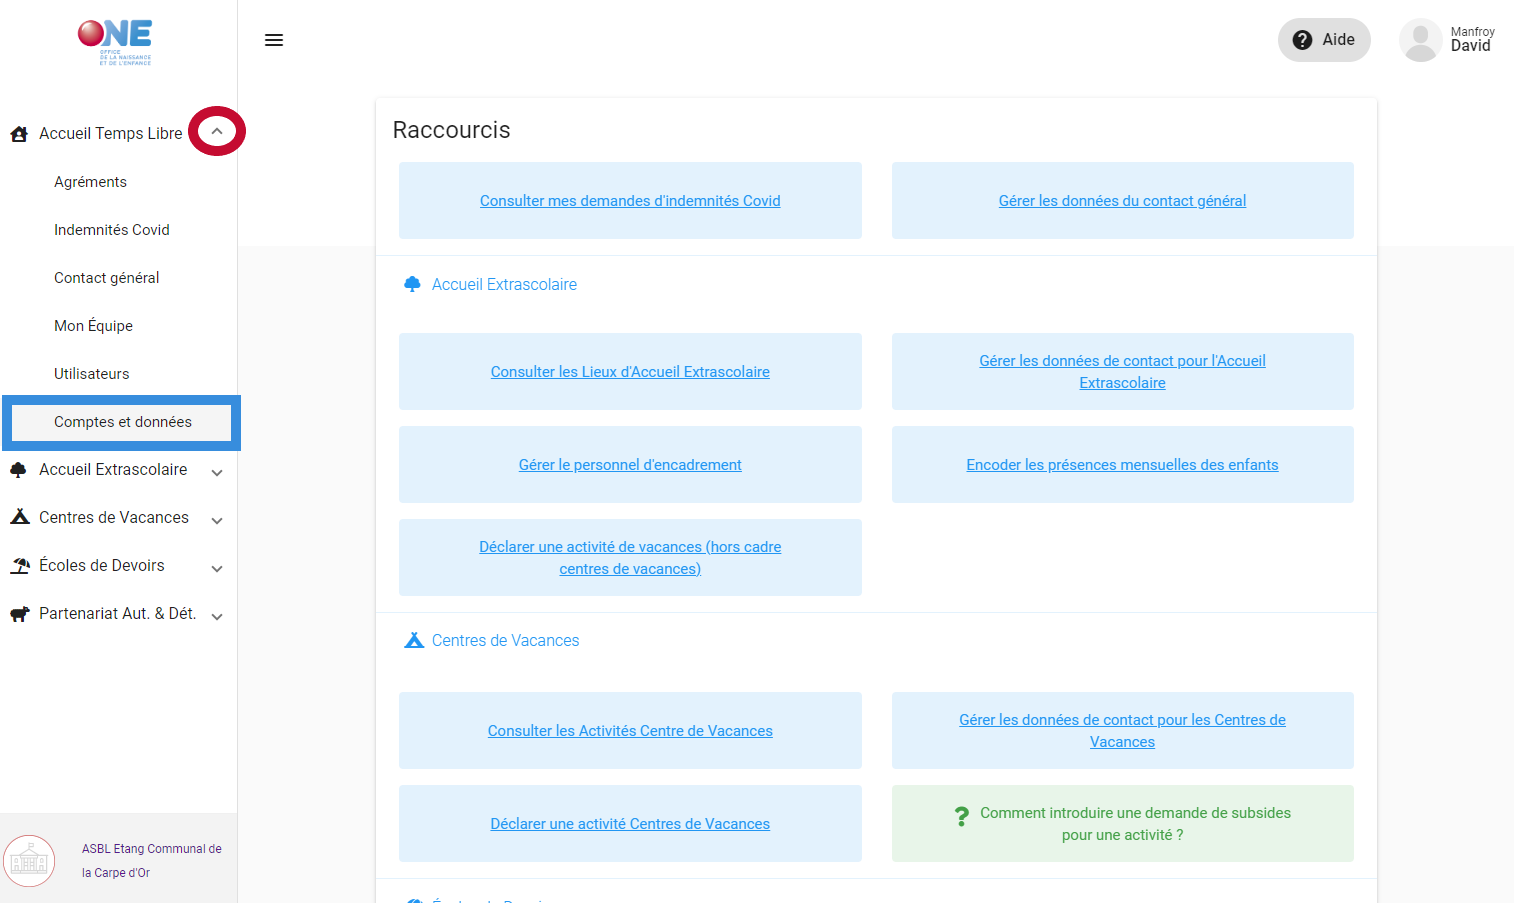
\includegraphics[width=0.95\textwidth]{Images/gcb/gcb_atlas.png}
         \caption{Dans le volet Accueil Temps Libre, cliquez sur l'entrée Comptes et Données}
         \label{subfig:gcb_atlas}
     \end{subfigure}
     \hfill
    \begin{subfigure}[t]{0.48\textwidth}
         \centering
         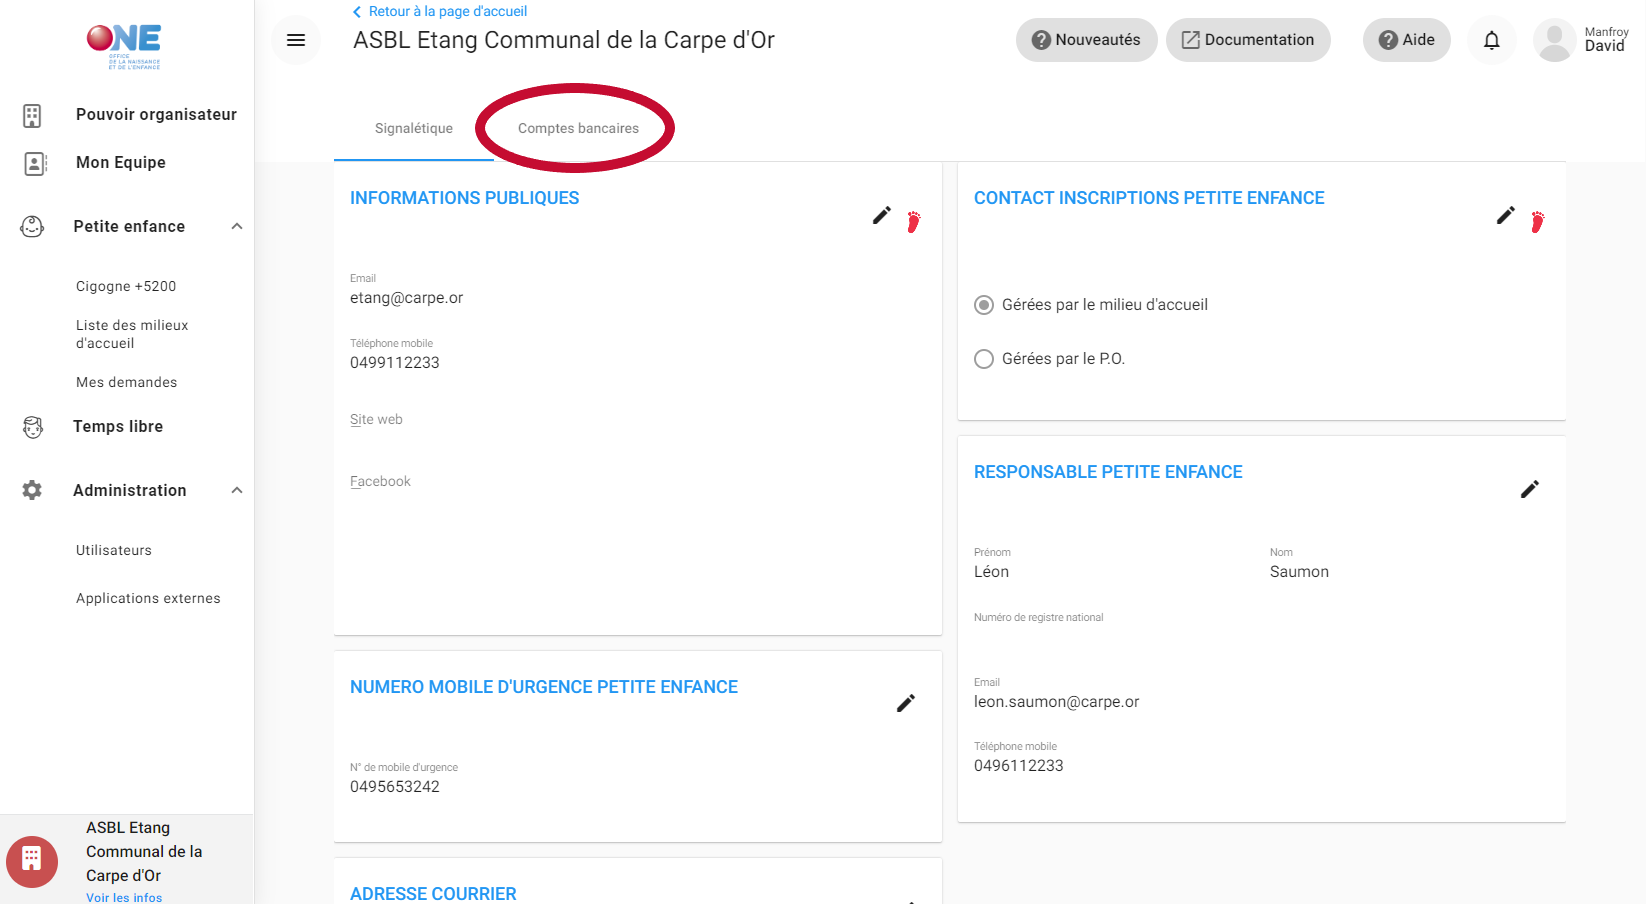
\includegraphics[width=0.95\textwidth]{Images/gcb/gcb_signaletique.png}
         \caption{Dans la signalétique du Pouvoir organisateur, cliquez sur "Comptes Bancaires"}
         \label{subfig:gcb_signalétique}
     \end{subfigure}
    
    \caption{Se rendre dans la gestion de vos comptes bancaires}
    \label{fig:gcb_atlas}
\end{figure}

\begin{attention}
Si vous souhaitez ajouter ou modifier un compte bancaire, vous devez TOUJOURS justifier celui-ci en soumettant un \textcolor{rouge}{relevé d’identité bancaire} que vous obtiendrez sur demande auprès de la banque à laquelle ce compte est relié.
\end{attention}

\subsection{Les types de compte}
\subsubsection{Compte principal}
Ce compte sera utilisé par défaut pour les payements de l'ONE.

\subsubsection{Compte(s) spécifique(s)}
Si vous utilisez plusieurs comptes, vous pouvez définir un compte pour le payement de vos subventions pour un secteur en particulier. Le payement se fera alors sur ce compte spécifique et non sur le compte principal.

\textbf{Finalité du compte}: lors de l'ajout (ou la modification) d'un compte spécifique, il vous sera alors demandé de préciser pour quel secteur le compte doit être utilisé. 

\textbf{Un seul compte par secteur}: un même compte spécifique peut être utilisé pour des secteurs différents. Cependant, vous ne pouvez avoir qu'un seul compte par secteur.

\subsection{Ajouter le compte bancaire par défaut}
Si vous n'avez pas de compte bancaire renseigné, un message dan un encadré jaune vous en avertis. Vous êtes invité à encoder le numéro IBAN du compte de votre structure. En cliquant sur le petit nuage, vous pourrez charger le relevé bancaire.

l'ONE validera ensuite le compte. Un petit V vous indiquera que le compte a été vérifié.
\subimport{Figures}{1.default_account}


\subsection{Ajouter un compte bancaire supplémentaire}
Pour ajouter un compte bancaire, vous pouvez cliquer sur \ovalbox{ + Ajouter un compte bancaire}. Dans la fenêtre d'ajout, ajoutez le numéro de compte.  Chargez ensuite la preuve de relevé d'identité bancaire (RIB). Sélectionnez enfin les secteurs pour lesquels le compte doit être utilisé. Vous pouvez sélectionner plusieurs finalités pour un même compte bancaire.

l'ONE validera ensuite le compte. Un petit V vous indiquera que le compte a été vérifié.



\subimport{Figures}{1.specific_account}

